\title{DBIx::Class Training}
\author{Stefan Hornburg (Racke), Peter Mottram (SysPete)}
\date{Perl Dancer Conference 2015, Vienna, 20th October 2015}

\begin{document}
\maketitle

\input sponsors.tex

\begin{frame}
  \titlepage
\end{frame}

\cleardoublepage

\tableofcontents

\cleardoublepage

\section{Introduction}

This training describes a sample application making use of
DBIx::Class and additional modules which makes you life
way easier. So first of all, we give you and idea what
the application is about.

\subsection{TravelDance Application}

You enjoy traveling, don't you? Even if not, we take you
along for a ride.

\begin{frame}{Traveling is Fun}
% https://pixabay.com/en/volkswagen-car-bus-mobile-home-158463/
\begin{figure}[!ht]
\centering

\includegraphics[width=1\linewidth]{img/volkswagen.png}
\end{figure}
\end{frame}

You can take this to another level, like doing a
competition between who visited the most countries:

% All images downloaded from Wikipedia

\begin{frame}{Countries}
\begin{figure}[!ht]
\centering

\begin{minipage}{.24\textwidth}
\centering

\includegraphics[width=1\linewidth]{img/countries/canada.png}
\caption{Canada}
\end{minipage}
% avoid paragraph break
\begin{minipage}{.24\textwidth}
\centering

\includegraphics[width=0.8\linewidth]{img/countries/austria.png}
\caption{Austria}
\end{minipage}
% avoid paragraph break
\begin{minipage}{.24\textwidth}
\centering

\includegraphics[width=0.8\linewidth]{img/countries/slovakia.png}
\caption{Slovakia}
\end{minipage}
% avoid paragraph break
\begin{minipage}{.24\textwidth}
\centering

\includegraphics[width=0.8\linewidth]{img/countries/usa.png}
\caption{USA}
\end{minipage}

\end{figure}

\end{frame}

\begin{frame}{Topics of Application}
\begin{itemize}
\item Countries
\item Users
\item Locations
\end{itemize}
\end{frame}

\begin{frame}{Locations}
\begin{itemize}
\item Country
\item User
\item Visited date
\item ...
\end{itemize}
\end{frame}

Of course there are already applications around to manage
your travel destinations.

%\note{
%I'm currently using TripAdvisor's app.
%}

\begin{frame}{Existing Applications}
\begin{itemize}
\item \sout{Privacy}
\item \sout{Options}
\item Slow
\end{itemize}
\end{frame}

\begin{frame}{Our Application}
\begin{itemize}
\item Fast
\item Privacy
\item Options
\end{itemize}
\end{frame}

\subsection{Database}
\begin{frame}{Database}
\centering
We need a database ...
\end{frame}

... something like that.

\begin{frame}{Database}
% https://pixabay.com/en/bottles-empty-glass-container-392689/
\begin{figure}[!ht]
\centering
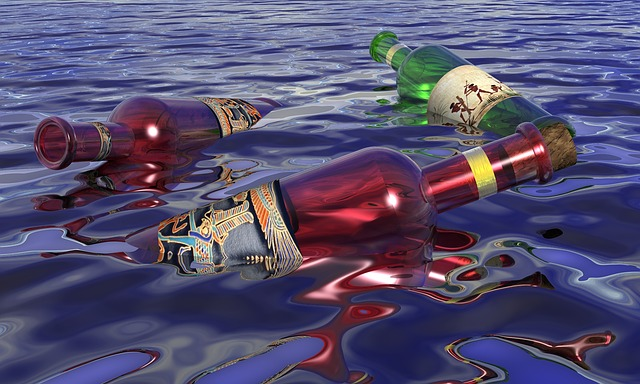
\includegraphics[width=1\linewidth]{img/bottles.jpg}
\end{figure}
\end{frame}

\begin{frame}{SQL is ...}
\begin{itemize}
\item SQL is ... boring
\item SQL is ... complex
\item SQL is ... incompatible
\end{itemize}
\end{frame}

\begin{frame}{Complex SQL query}
% add example for complex SQL query
\end{frame}

\begin{frame}{Squeeze OO}
% OO supplied by DBIx::Class
% DBIx::Class + Moo

Object relationship manager (ORM)
SQL => OO
hashref => 

\end{frame}

Just for the fun it, later you will learn how do you
use DBIx::Class to retrieve hash references instead of
objects!

\begin{frame}{DBIx::Class to the rescue!}
% DBIx::Class
\end{frame}

\begin{frame}{Business Logic}
% move business logic into schema
\end{frame}

\begin{frame}{Life Savers for DBIx::Class}
% https://pixabay.com/en/candy-cane-candy-cane-winter-488009/
\begin{figure}[!ht]
\centering

\includegraphics[width=0.8\linewidth]{img/candy-cane.jpg}
\end{figure}
\end{frame}

\subsection{Starting with DBIx::Class}

\begin{frame}{Starting with DBIx::Class}
\begin{itemize}
\item Existing project
\item New project
\end{itemize}
\end{frame}

\subsubsection{Existing Project}

You can use \verb|dbicdump| to create a ``boilerplate'' schema from the
existing database.

\begin{frame}[fragile]{dbicdump}
\begin{lstlisting}
dbicdump -o dump_directory=/home/dance/TravelDance/lib 
         TravelDance::Schema 
         dbi:Pg:dbname=perldance
\end{lstlisting}
\end{frame}

\verb|dbicdump| also provides additional options, e.g.
including \verb|DBIx::Class| components, which we cover
later in the training.

\begin{frame}[fragile]{dbicdump with Components}
\begin{lstlisting}
dbicdump -o dump_directory=/home/dance/TravelDance/lib 
         -o components='["InflateColumn::DateTime"]'
         TravelDance::Schema 
         dbi:Pg:dbname=perldance
\end{lstlisting}
\end{frame}

\subsubsection{Creating database}
Starting a new project involves creating a database, which
isn't as simple as you would think.

MySQL databases should be created with UTF8 encoding and appropriate 
collation for your local, for example:

\begin{frame}[fragile]{Creating MySQL database}
\begin{lstlisting}
    CREATE DATABASE "my_shop_db"
        DEFAULT CHARACTER SET utf8
        DEFAULT COLLATE utf8_general_ci;
\end{lstlisting}
\end{frame}

The following L<Connection attributes|DBIx::Class::Storage::DBI/DBIx::Class specific connection attributes> are recommended as a minimum for MySQL:

\begin{frame}[fragile]{MySQL Connection attributes}
\begin{lstlisting}
    mysql_enable_utf8 => 1,
    on_connect_do     => [
        q|SET SQL_MODE = CONCAT('ANSI,TRADITIONAL,', @@sql_mode)|,
        q|SET SQL_AUTO_IS_NULL = 0|,
    ],
\end{lstlisting}
\end{frame}

NOTE: we no longer recommend the use of 
\verb|on_connect_call =>'set_strict_mode'| since that also forces MySQL's 
\href{https://dev.mysql.com/doc/refman/5.0/en/sql-mode.html#sqlmode\_only\_full\_group\_by}{ONLY\_FULL\_GROUP\_BY} mode which prevents us from using GROUP BY on PK columns which is a great performance boost for PostgreSQL.

=head1 PostgreSQL

PostgreSQL databases should be created with UT8 encoding, for example:

\begin{frame}[fragile]{Creating PostgreSQL database}
\begin{lstlisting}
    createdb -E UTF8 my_shop_db
\end{lstlisting}
\end{frame}

The following L<Connection attributes|DBIx::Class::Storage::DBI/DBIx::Class specific connection attributes> are recommended as a minimum for PostgreSQL:

\begin{frame}[fragile]{PostgreSQL Connection attributes}
\begin{lstlisting}
    pg_enable_utf8 => 1,
    on_connect_do  => 'SET client_min_messages=WARNING;',
\end{lstlisting}
\end{frame}

\section{DBIC Classes}

\begin{frame}{DBIC Classes}
\begin{itemize}
\item Two mandatory types of class
\item One schema class
\begin{itemize}
\item TravelDance::Schema
\end{itemize}
\item One result class for each table
\begin{itemize}
\item TravelDance::Schema::Result::Country
\item TravelDance::Schema::Result::Location
\item TravelDance::Schema::Result::User
\end{itemize}
\end{itemize}
\end{frame}

\subsection{Schema Class}

Here we see the minimal DBIx::Class schema definition:

\begin{frame}[fragile]{Schema Class}
\begin{lstlisting}
package TravelDance::Schema;
use warnings;
use strict;
use base 'DBIx::Class::Schema';

__PACKAGE__->load_namespaces();
1;
\end{lstlisting}
\end{frame}

\verb|load_components| searches \verb|TravelDance::Schema::Result{Set}::*|
for Result and ResultSet classes and loads them into the schema.

\subsection{Result Classes}

\begin{frame}{Result Classes}
\begin{itemize}
\item Need one result class for each table
\item Country => countries
\item Location => locations
\item User => users
\end{itemize}
\end{frame}

\subsubsection{Result Class Definition}
Describes each result class and the database table behind it. 

See \href{https://metacpan.org/pod/DBIx::Class::ResultSource}{DBIx::Class::ResultSource} for more details.

\begin{frame}{Result Class Definition}

\begin{itemize}
\item Table name
\item Columns
\item Primary key
\item Relationships
\end{itemize}
\end{frame}

\subsection{Country Result Class}

\begin{frame}[fragile]{Country / Vanilla DBIx::Class}
\begin{lstlisting}
package TravelDance::Schema::Result::Country;
use base qw/DBIx::Class::Core/;
__PACKAGE__->add_columns(
    country_iso_code => {
        data_type => "char",
        size      => 2,
    },
    name => {
        data_type => "varchar",
        size      => 255,
    },
);
\end{lstlisting}
\end{frame}

\begin{frame}[fragile]{Country / Vanilla DBIx::Class}
\begin{lstlisting}
__PACKAGE__->set_primary_key("country_iso_code");

__PACKAGE__->has_many(
    locations =>
      "TravelDance::Schema::Result::Location",
      'country_iso_code'
);

__PACKAGE__->many_to_many(
    users => "locations", "user"
);
\end{lstlisting}
\end{frame}

\begin{frame}[fragile]{Country / DBIx::Class::Candy}
\begin{lstlisting}
package TravelDance::Schema::Result::Country;
use TravelDance::Schema::Candy;

primary_column country_iso_code => {
    data_type => "char",
    size      => 2
};

column name => {
    data_type => "varchar",
    size      => 255
};
\end{lstlisting}
\end{frame}

\begin{frame}[fragile]{Country / DBIx::Class::Candy}
\begin{lstlisting}
has_many
  locations =>
  "TravelDance::Schema::Result::Location",
  'country_iso_code';

many_to_many users => "locations", "user";
\end{lstlisting}
\end{frame}

\subsection{Location Result Class}

\begin{frame}[fragile]{User / Vanilla DBIx::Class}
\begin{lstlisting}

\end{lstlisting}
\end{frame}

\begin{frame}[fragile]{User / DBIx::Class::Candy}
\begin{lstlisting}
package TravelDance::Schema::Result::Location;
use TravelDance::Schema::Candy;

primary_column locations_id => {
    data_type         => "integer",
    is_auto_increment => 1,
};
column address => {
    data_type     => "varchar",
    default_value => "",
    size          => 255,
};
\end{lstlisting}
\end{frame}

\begin{frame}[fragile]{User / DBIx::Class::Candy}
\begin{lstlisting}
column address_2 => {
    data_type     => "varchar",
    default_value => "",
    size          => 255,
};

column postal_code => {
    data_type     => "varchar",
    default_value => "",
    size          => 255,
};
\end{lstlisting}
\end{frame}

\begin{frame}[fragile]{User / DBIx::Class::Candy}
\begin{lstlisting}
column city => {
    data_type     => "varchar",
    default_value => "",
    size          => 255,
};

column region => {
    data_type     => "varchar",
    default_value => "",
    size          => 255,
};
\end{lstlisting}
\end{frame}

\begin{frame}[fragile]{User / DBIx::Class::Candy}
\begin{lstlisting}
column country_iso_code => {
    data_type      => "char",
    size           => 2,
    is_nullable    => 1,
};

column visited => {
    data_type     => "datetime",
};
\end{lstlisting}
\end{frame}

\begin{frame}[fragile]{User / DBIx::Class::Candy}
\begin{lstlisting}
column users_id => {
    data_type      => "integer",
};

belongs_to
  country => "TravelDance::Schema::Result::Country",
  "country_iso_code", { join_type => 'left' };

belongs_to user => "TravelDance::Schema::Result::User",
  "users_id";
\end{lstlisting}
\end{frame}

% \subsection{User Result Class}

% \begin{frame}[fragile]{User / Vanilla DBIx::Class}
% \begin{lstlisting}

% \end{lstlisting}
% \end{frame}

% \begin{frame}[fragile]{User / DBIx::Class::Candy}
% \begin{lstlisting}

% \end{lstlisting}
% \end{frame}

\section{CRUD and Beyond}
\begin{frame}{CRUD and Beyond}
\end{frame}

\subsection{CRUD}

CRUD is defined as:

\begin{frame}{CRUD}
\begin{description}
\item[C] - Create
\item[R] - Retrieve
\item[U] - Update
\item[D] - Delete
\end{description}
\end{frame}

\subsubsection{C - Create}
\begin{frame}[fragile]{C - Create}
Create in the simplest form:

\begin{lstlisting}
my $user = $schema->resultset('User')->create(
    {
        username => 'syspete',
        email    => 'syspete@example.com',
        password => 're@llybadpwd',
    }
);
\end{lstlisting}
\end{frame}

Tip: do not pass in primary key field if it is auto-increment since that will be added automatically.

\subsubsection{C++ - Multi Create}
It's even possible to create an user and corresponding locations at the
same time:

\begin{frame}[fragile]{C++ - Multi Create}
\begin{lstlisting}
my $user = $schema->resultset('User')->create(
    {
        email    => 'syspete@example.com',

        locations => [
            {
                country_iso_code => 'DE',
                city => 'Hannover',
            },
            {
                country_iso_code => 'AT',
                city => 'Vienna',
            },
        ],
    }
);
\end{lstlisting}
\end{frame}

\subsubsection{U - Update}

One row only:

\begin{frame}[fragile]{U - Update (one row)}
\begin{lstlisting}
$user->update({
        email => 'syspete@newdomain.com'
});
\end{lstlisting}
\end{frame}

You can also use the column accessor then force the update to be pushed to
the database:

\begin{frame}[fragile]{U - Update (through accessor)}
\begin{lstlisting}
$user->email('syspete@newdomain.com');
$user->update;
\end{lstlisting}
\end{frame}

Many rows in a table:

\begin{frame}[fragile]{U - Update (multiple rows)}
\begin{lstlisting}
my $rs = $schema->resultset('User')->search(...);
$rs->update({ fail_count => 0 });
\end{lstlisting}
\end{frame}

\subsubsection{D - Delete}

One row only:

\begin{frame}[fragile]{D - Delete (one row)}
\begin{lstlisting}
$user->delete;
\end{lstlisting}
\end{frame}

Many rows in a table:

\begin{frame}[fragile]{D - Delete (multiple rows)}
\begin{lstlisting}
my $rs = $schema->resultset('User')->search(...);
$rs->delete;
\end{lstlisting}
\end{frame}

\subsection{Chaining}
% from riba's slides

\begin{frame}{Chaining}
  \begin{figure}[!ht]
    \begin{center}
      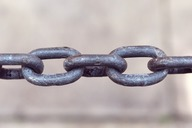
\includegraphics{img/chains.jpg}
      \caption[Chains]{Picture from Katrin Baustmann}
    \end{center}
  \end{figure}
\end{frame}

% picture from
% https://pixabay.com/en/chain-chain-link-border-demarcation-722278/
% Creative Commons CC0

\subsubsection{Shallow Nesting (Chaining)}

\begin{frame}[fragile]{Shallow Nesting (Chaining)}
\begin{lstlisting}
    $rs->search({ name => { '!=', 'blah' }})
        ->search({ name => { '!=', undef }})

    ... WHERE name != 'blah' AND name IS NOT null
\end{lstlisting}
\end{frame}

\subsubsection{Subquery nesting}

\begin{frame}[fragile]{Subquery nesting}
\begin{lstlisting}
    $rs->search({}, { distinct => 1 })
        ->as_subselect_rs
         ->search({}, { rows => 1 })

    ... SELECT FROM (SELECT * FROM artist GROUP_BY * )
        LIMIT 1
\end{lstlisting}
\end{frame}

\subsection{Correlated Subqueries}
\begin{frame}{Correlated Subqueries}
\end{frame}

\section{Using relationships}

\begin{frame}{Using relationships}
\begin{itemize}
\item has\_many, might\_have and has\_one
\item many\_to\_many
\item Relationship conditions
\item Relationship attributes
\item Relationships with nullable FKs
\end{itemize}
\end{frame}

\subsection{has\_many, might\_have and has\_one}

In DBIx::Class a relationship defines the connection between exactly two
tables. The relationship condition lists the columns in each table that
contain the same values. It is used to output an SQL JOIN condition between
the tables.

One side of the relationship is always a \verb|belongs_to| relationship
where the calling class stores the stores the foreign class’s primary key in
one (or more) of the calling class columns.

In our example schema every user can have zero, one or many locations and
each Location \verb|belongs_to| a single User so we have the following column and
relationship defined in the Location class: 
 
\begin{frame}[fragile]{belongs\_to}
\begin{lstlisting}
column users_id => {
    data_type      => "integer",
};

belongs_to
  user => "TravelDance::Schema::Result::User",
  { 'foreign.users_id' => 'self.users_id' };
\end{lstlisting}
\end{frame}

Here ‘user’ is the name of the relationship and also the name of the relationship accessor that is created. The second argument is the foreign class and the final argument is the relationship condition. Here we have a simple equality condition.

Note the use of ‘is\_foreign\_key’ in the users\_id column definition. This is used when the schema is deployed and instructs SQL::Translator to create the appropriate foreign key constraints in the database.

In the User class we define the primary key which is referenced by the Location class::

\begin{frame}[fragile]{Primary key}
\begin{lstlisting}
primary_column users_id => {
    data_type         => "integer",
    is_auto_increment => 1,
};
\end{lstlisting}
\end{frame}

And since we expect each user to have many locations we define the relationship as a \verb|has_many|:

\begin{frame}[fragile]{Locations Relationship}
\begin{lstlisting}
has_many locations =>
  "TravelDance::Schema::Result::Location",
  { 'foreign.users_id' => 'self.users_id' };
\end{lstlisting}
\end{frame}

Note: has\_many does not mean that there must be many related items but only that there can be many. One or zero related items is also possible (a LEFT JOIN).


\begin{frame}{has\_many / might\_have}
\begin{table}
\begin{tabular}{c | c | c}
relationship type & default join type & number of related rows \\
\hline
has\_many & LEFT & zero, one or many \\
might\_have & LEFT & zero or one \\
\end{tabular}
\end{table}
\end{frame}

The difference here is that with a collapsed search (to be covered later)
the has\_many accessor returns a resultset whereas the might\_have accessor
returns a result object (a single row).

\subsection{many\_to\_many}

This is not a relationship but a convenience method generator which defines an
accessor to retrieve row contents across multiple relationships.

The difference between a bridge and a relationship is, that the bridge
cannot be used to join tables in a search, instead its component
relationships must be used.

\subsection{Relationship conditions}

\begin{frame}{Relationship conditions}
\begin{itemize}
\item Simple equality
\item Multiple groups of simple equality conditions
\item Custom join conditions
\end{itemize}
\end{frame}

\subsubsection{Simple equality}

Simple equality conditions
in User:

\begin{frame}[fragile]{Simple equality conditions}
\begin{lstlisting}
has_many
  locations => "TravelDance::Schema::Result::Location",
  { 'foreign.users_id' => 'self.users_id' };
\end{lstlisting}
\end{frame}

If the column has the same name in both tables then the condition can be replaced with the column name:

\begin{frame}[fragile]{Simple equality conditions}
\begin{lstlisting}
has_many
  locations => "TravelDance::Schema::Result::Location",
  'users_id';
\end{lstlisting}
\end{frame}

\subsubsection{Multiple groups of simple equality conditions}

As is the default in SQL::Abstract, the key-value pairs will be ANDed in the
resulting JOIN clause. An OR can be achieved with an arrayref. For example a
condition like:

\begin{frame}[fragile]{Multiple groups of simple equality conditions}
\begin{lstlisting}
has_many
  related_item_links => "My::Schema::Item::Links",
  [
    { 'foreign.left_itemid'  => 'self.id' },
    { 'foreign.right_itemid' => 'self.id' },
  ];
\end{lstlisting}
\end{frame}

\subsubsection{Custom join conditions}

All locations visited before 1st January 2000.

\begin{frame}[fragile]{Custom join conditions}
\begin{lstlisting}
has_many
 before_2000 => "TravelDance::Schema::Result::Location",
 sub {
   my $args = shift;
   return {
      "$args->{foreign_alias}.users_id" =>
          { -ident => "$args->{self_alias}.users_id" },
      "$args->{foreign_alias}.visited" =>
          { '<', '2000-01-01' },
   };
 };
\end{lstlisting}
\end{frame}

\subsection{Relationship attributes}

% NOTE: we should mention these but not go into any detail except for join_type.

\begin{frame}{Relationship attributes}
\begin{itemize}
\item join\_type
% \item proxy => \verb|$column| | \verb|\@columns| | \verb|\%column|
\item accessor
\item is\_foreign\_key\_constraint
\item cascade\_copy / cascade\_delete / cascade\_update
\item on\_delete / on\_update
\item is\_deferrable
\item add\_fk\_index
\end{itemize}
\end{frame}

\subsection{Relationships with nullable FKs}

% Source for description: https://en.wikipedia.org/wiki/Marie_Byrd_Land
% License for Picture: CC BY 2.0 via Commons 

\subsubsection{Unclaimed Land}

Because of its remoteness, even by Antarctic standards, most of Marie Byrd
Land (the portion east of 150\degree{}W) has not been claimed by any sovereign
nation. It is by far the largest single unclaimed territory on Earth, with
an area of 1,610,000 km2 (620,000 sq mi) (including Eights Coast,
immediately east of Marie Byrd Land).

\begin{frame}{Unclaimed Land}
  \begin{figure}[!ht]
    \begin{center}
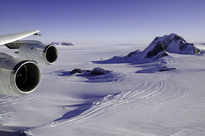
\includegraphics{img/Marie_Byrd_Land.jpg}
\caption[Marie Byrd Land]{Photo by Michael Studinger / NASA
  Goddard Space Flight Center}
    \end{center}
\end{figure}
\end{frame}

\subsubsection{Location without a country}

A location usually has a country but not if it is in a neutral zone like in
the middle of an ocean so this column is nullable:

\begin{frame}[fragile]{Location without a country}
\begin{lstlisting}
column country_iso_code => {
    data_type      => "char",
    size           => 2,
    is_nullable    => 1,
};
\end{lstlisting}
\end{frame}

Location has a belongs\_to relationship with Country and the default join
type for this relationship is an INNER JOIN (the default JOIN type) which
skips rows from the left-hand table if there is no corresponding row in the
right-hand table. Compare these two SQL queries and their result: 

\begin{frame}[fragile]{SQL queries}
\begin{lstlisting}
SELECT count(*) FROM locations l JOIN countries c
    ON l.country_iso_code=c.country_iso_code;
27

SELECT count(*) FROM locations l LEFT JOIN countries c
    ON l.country_iso_code=c.country_iso_code;
28
\end{lstlisting}
\end{frame}

So we use the join\_type relationship attribute in the relationship definition to force a LEFT JOIN:

\begin{frame}[fragile]{LEFT JOIN join\_type}
\begin{lstlisting}
belongs_to
  country => "TravelDance::Schema::Result::Country",
  "country_iso_code",
  { join_type => 'left' };
\end{lstlisting}
\end{frame}

\section{Extending Schema}
\begin{frame}{Extending Schema}
\begin{itemize}
\item Result Class Components
\item Helpers
\end{itemize}
\end{frame}

\subsection{Using Result Class Components}

In a single result class:

\begin{frame}[fragile]{Using Components}
\begin{lstlisting}
package TravelDance::Schema::Result::User;

use TravelDance::Schema::Candy -components => [qw(
    InflateColumn::DateTime 
    PassphraseColumn
    TimeStamp
)];
\end{lstlisting}
\end{frame}

To add a result class component to all result classes add to list 
in \verb|TravelDance::Schema::Candy|'s \verb|parse_arguments|.

\subsubsection{Password/passphrase columns}

DBIx::Class::PassphraseColumn uses the column definition when hashing a new
password/passphrase but can test the password against many types of hash
stored in the column. This allows an application to switch from (say)
MD5 crypt to blowfish whilst still working with the old hashes.

\begin{frame}[fragile]{Password column}
\begin{lstlisting}
column password => {
    data_type        => "text",
    default_value    => "",
    passphrase       => 'crypt',
    passphrase_class => 'BlowfishCrypt',
    passphrase_args  => {
        cost        => 14,
        key_nul     => 1,
        salt_random => 1,
    },
    passphrase_check_method => 'check_password',
};
\end{lstlisting}
\end{frame}

\subsubsection{Automatic setting of date/datetime columns on create/update}
DBIx::Class::TimeStamp

From User class:

\begin{frame}[fragile]{Create/update date columns}
\begin{lstlisting}
column created => {
    data_type     => "datetime",
    set_on_create => 1,
};


column last_modified => {
    data_type     => "datetime",
    set_on_create => 1,
    set_on_update => 1,
};
\end{lstlisting}
\end{frame}

\subsubsection{Automatic DateTime inflation from columns}

Using DBIx::Class::InflateColumn::DateTime we can have date and datetime
columns automatically converted to DateTime objects when retrieved from the
database. The reverse also happens and DateTime objects are converted back
into a format appropriate for the underlying database engine on
create/update.

NOTE: Don't rely on InflateColumn::DateTime to parse date strings for
you. The column is set directly for any non-references and
InflateColumn::DateTime is completely bypassed. For example if you pass a
string value date directly to create/update then this will be stored AS IS
and on retrieve might be in a format that InflateColumn::DateTime’s inflator
does not understand resulting in an exception rather than the DateTime
object you are expecting. The rule is always pass DateTime objects when
creating/updating a column with this inflator set. 

\subsection{Helpers}
\subsubsection{ResultSet Helpers}
\begin{description}
\item[Me] 
simple exact way to set table aliases correctly in queries
\item[Random] small random subset
great for related product searches where you want a small 
random subset of the results
\item[CorrelateRelationship] 
makes correlated subqueries really simple
\end{description}

\begin{frame}{ResultSet Helpers}
\begin{description}
\item[Me] correct table aliases
\item[Random] small random subset
\item[CorrelateRelationship]  
\end{description}
\end{frame}

\begin{frame}{CorrelateRelationship}

Problem: we want a count of rows in a related table

\end{frame}

So the obvious approach for this is:

\begin{frame}[fragile]{CorrelateRelationship}
\begin{lstlisting}
    my $rs = $schema->resultset('Author')->search(
        undef,
        {
            join       => 'books',
            '+columns' => {
                book_count => {
                    count => 'books.id'
                }
            },
            distinct   => 1,    # let DBIC work out group_by for us
        }
    );
\end{lstlisting}
\end{frame}
This causes a number of problems:

\begin{itemize}
\item Depending on engine, COUNT’s that aren’t COUNT(*) tend to be slow as
they do table scans.
\item This is hard to chain since we've introduced JOIN and GROUP BY and
collapsed COUNTs might produced unexpected results.
\item We cannot add other interesting data from the locations in the same query (such as date of most recent visit).
\end{itemize}

\begin{frame}[fragile]{CorrelateRelationship}
\begin{lstlisting}
Much nicer to do:

    package MyApp::Schema::ResultSet::Author;

    use parent 'DBIx::Class::ResultSet';

   
__PACKAGE__->load_components(qw(Helper::ResultSet::CorrelateRelationship));

    sub with_book_count {
        my $self = shift;

        $self->search(
            undef,
            {
                '+columns' => {
                    book_count =>
$self->correlate('books')->count_rs->as_query
                }
            }
        );
    }
\end{lstlisting}
\end{frame}

\begin{frame}[fragile]{CorrelateRelationship}
Then elsewhere:

\begin{lstlisting}
my $rs = $schema->resultset('Author')->with_book_count;

The SQL query will look something like this:

  SELECT me.id, me.name, me.foo, ..., (
    SELECT COUNT( * )
      FROM books books_alias
     WHERE books_alias.id = authors.id
   )
  FROM authors me

This is *much* faster and *always* chainable since no JOIN, GROUP BY, or
other junk added to query.
\end{lstlisting}
\end{frame}

Cool example from Interchange6::Schema::ResultSet::Product :

\begin{lstlisting}
    sub with_average_rating {
        my $self = shift;

        return $self->search(
            undef,
            {
                '+select' => [
                    {
                        coalesce => [

                            $self->correlate('canonical')
                              ->related_resultset('_product_reviews')
                              ->search_related(
                                'message',
                                { 'message.approved' => 1,
'message.public' => 1 }
                             
)->get_column('rating')->func_rs('avg')->as_query,

                            $self->correlate('_product_reviews')
                              ->search_related(
                                'message',
                                { 'message.approved' => 1,
'message.public' => 1 }
                             
)->get_column('rating')->func_rs('avg')->as_query,

                          ],
                        -as => 'average_rating'
                    }
                ],
                '+as' => ['average_rating'],
            }
        );
    }
\end{lstlisting}

\subsubsection{Shortcuts}
\begin{description}
\item[AddColumns] 
\item[Columns]
\item[Distinct]
\item[GroupBy] 
\item[HRI]
uses this all the time
\item[HasRows] much faster than count for very large resultsets
\item[Limit]
\item[OrderBy]
\item[Page]
\item[Prefetch]
\item[Rows]
\item[Search::{Not}Like]
\item[Search::{Not}Null] 
\end{description}

Using the HashRefInflator makes sense when you need to quickly retrieve
data from a massive resultset or you need a list of hash references anyway,
e.g. for input to a template in a web application.

\begin{frame}[fragile]{HashRefInflator}
\begin{lstlisting}
my $rs = $schema->resultset('Country')->search({}, {
   result_class
     => 'DBIx::Class::ResultClass::HashRefInflator',
 });
\end{lstlisting}
\end{frame}

\begin{frame}[fragile]{HashRefInflator with HRI helper}
\begin{lstlisting}
my $rs = $schema->resultset('Country')->search({})->hri;

# since 'search' here is redundant we can just use:
my $rs = $schema->resultset('Country')->hri;
\end{lstlisting}
\end{frame}

\subsubsection{Schema}
\begin{description}
\item[DateTime]
much simpler query construction for DateTime inflated fields
\item[QuoteNames] 
forces quote\_names even if someone misses it in their 
config yml - everyone should use this
\end{description}

\begin{frame}{Schema Helpers}
\begin{description}
\item[DateTime] DateTime inflated fields
\item[QuoteNames] forces quote\_names
\end{description}
\end{frame}

% \section{Writing Tests}
% \begin{frame}{Writing Tests}
% \end{frame}

\section{Deployment Handler}

\subsection{Deploy/Upgrade/Downgrade}

\begin{frame}{Deployment Handler}
\begin{itemize}
\item DBIx::Class::DeploymentHandler
\item Deploy databases
\item Upgrade databases
\item Downgrade databases
\end{itemize}
\end{frame}

\subsection{Principles}

\begin{frame}{Principles}
\begin{itemize}
\item Create backup
\item Change schema
\item Add custom scripts
\item Bump version number
\item Prepare upgrade
\item Deploy upgrade
\end{itemize}
\end{frame}

Note: create backup can be done by DeploymentHandler itself.

\subsection{Change Schema}

\begin{frame}{Change Schema}
\begin{itemize}
\item Add table
\item Add column
\item Alter column
\end{itemize}
\end{frame}

\subsection{Bump version number}
\begin{frame}{Bump version number}
\begin{itemize}
\item Natural number => 1
\item Increase by 1 => 2
\end{itemize}
\end{frame}

\begin{frame}[fragile]{Version 1}
\begin{lstlisting}
package TravelDance::Schema;
use warnings;
use strict;
use base 'DBIx::Class::Schema';

our $VERSION = 1;

__PACKAGE__->load_namespaces();

1;
\end{lstlisting}
\end{frame}

\begin{frame}[fragile]{Version 2}
\begin{lstlisting}
package TravelDance::Schema;
use warnings;
use strict;
use base 'DBIx::Class::Schema';

our $VERSION = 2;

__PACKAGE__->load_namespaces();

1;
\end{lstlisting}
\end{frame}

\subsection{Prepare upgrade}

\begin{frame}[fragile]{Prepare upgrade}
\begin{lstlisting}
my $dh     = DBIx::Class::DeploymentHandler->new(
    {
        schema              => $schema,
        databases           => 'MySQL',
        sql_translator_args => { add_drop_table => 0 }
    }
);
$dh->prepare_deploy;
$dh->prepare_upgrade(
    {
        from_version => $dh->database_version,
        to_version => $dh->schema_version
    }
);
\end{lstlisting}
\end{frame}

\subsection{Add custom scripts}

\begin{frame}{Add custom scripts}
\begin{itemize}
\item Add initial values for new tables
\begin{itemize}
\item hardcoded in script
\item from file
\end{itemize}
\end{itemize}
\end{frame}

\subsection{Internals}

\begin{frame}{Directories and files}
\end{frame}

\end{document}

%%% Local Variables: 
%%% mode: latex
%%% TeX-master: t
%%% End: 
